\documentclass{beamer}
\usetheme{Montpellier}
\usecolortheme{beaver}
\usepackage{verbatim}	
\usepackage[square,sort]{natbib}
\usepackage{comment}
\usepackage{amsmath}
\usepackage{caption}


\setbeamerfont{footnote}{size=\tiny}
\setbeamerfont{footnote mark}{size=\tiny}
\setbeamerfont{caption}{size=\scriptsize}
\setbeamerfont{cite}{size=\tiny}


\title{X-ray wave propagation in PETSc }
\author{Sajid Ali\inst{1} \& Chris Jacobsen\inst{2}}	
\institute[NU] 
{\inst{1}%
  Applied Physics\\
  Northwestern University\\
\inst{2}%	
	X-ray Science Divison\\
	Argonne National Lab}
\date{\today}
% If you have a file called "university-logo-filename.xxx", where xxx
% is a graphic format that can be processed by latex or pdflatex,
% resp., then you can add a logo as follows:

% \pgfdeclareimage[height=0.5cm]{university-logo}{university-logo-filename}
% \logo{\pgfuseimage{university-logo}}

% Delete this, if you do not want the table of contents to pop up at
% the beginning of each subsection:
\AtBeginSubsection[]
{
  \begin{frame}<beamer>{Outline}
    \tableofcontents[currentsection,currentsubsection]
  \end{frame}
}
\AtBeginSection[]{
	\begin{frame}
		\vfill
		\centering
		\begin{beamercolorbox}[sep=8pt,center,shadow=true,rounded=true]{title}
			\usebeamerfont{title}\insertsectionhead\par%
		\end{beamercolorbox}
		\vfill
	\end{frame}
}

% Let's get started
\begin{document}


\begin{frame}
  \titlepage
\end{frame}

\begin{frame}{Outline}
  \tableofcontents
  % You might wish to add the option [pausesections]
\end{frame}

% Section and subsections will appear in the presentation overview
% and table of contents.
\section{Introduction}
\begin{frame}{Synchrotron light sources}
	\begin{itemize}
	\item Accelerate electrons close to speed of light, then bend the beam to produce ''bright'' x-rays.
		\begin{center}
		\begin{figure}
			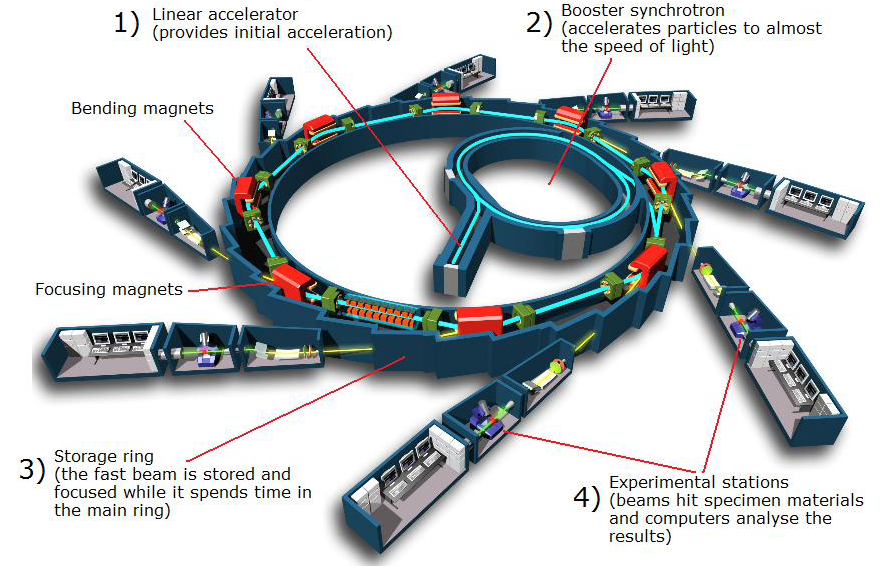
\includegraphics[scale=0.3]{synchrotron}
			\caption{Synchtrotron schematic\footnote{\url{https://dc.edu.au/hsc-physics-quanta-to-quarks/}}}	
		\end{figure}
		\end{center}
	\end{itemize}
\end{frame}

\begin{frame}{More than Moore! \footnote{\cite{synchrotron}}}
	%\begin{itemize}
		%\item Synchrotron brightness has been increasing faster than Moore's law \cite{synchrotron}.
		\begin{center}
		\begin{figure}
			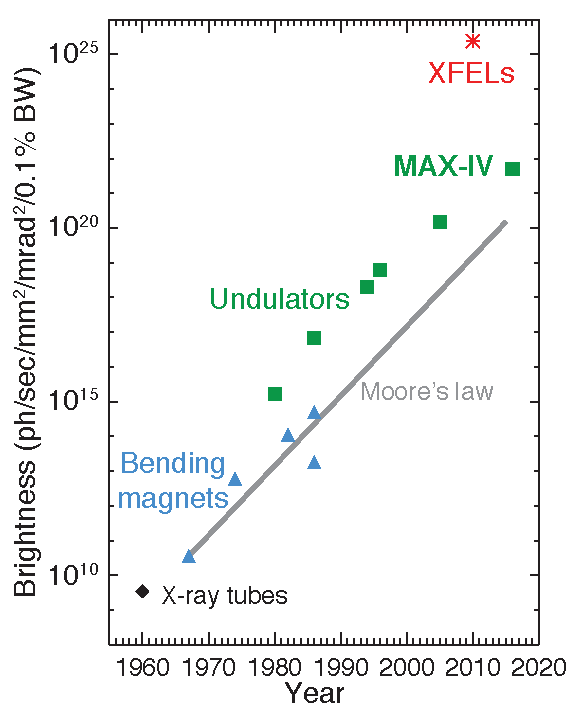
\includegraphics[scale=0.55]{xray}
		\end{figure}
		\end{center}	
	%\end{itemize}
\end{frame}


\section{Zone Plates}

\begin{frame}{Focusing X-Rays}
	\begin{block}{}
		\begin{columns}[onlytextwidth,T]
			\column{\dimexpr\linewidth-30mm-10mm}
			\begin{itemize}
			\item Ref. index$\rightarrow$ complex,slightly $<$ 1
			\item Zone plates$\rightarrow$ monochromatic diffractive optics.
			\item Consist of alternate rings of low and high refractive index materials placed such that the outgoing waves constructively interfere with each other at the focal spot.
			\end{itemize}
			\column{30mm}
			\begin{figure}
				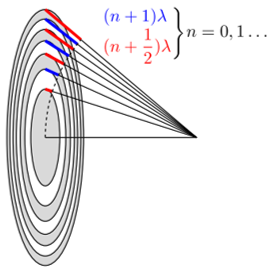
\includegraphics[width=40mm]{zp}
				\caption{Illustration of zone plate \footnotemark}
			\end{figure}
		\end{columns}
	\footnotetext{\cite{jacobsen_2019}}
	\end{block}
\end{frame}

\begin{frame}{Zone plates in action!}
	%\begin{itemize}
		\begin{center}
			\begin{figure}
				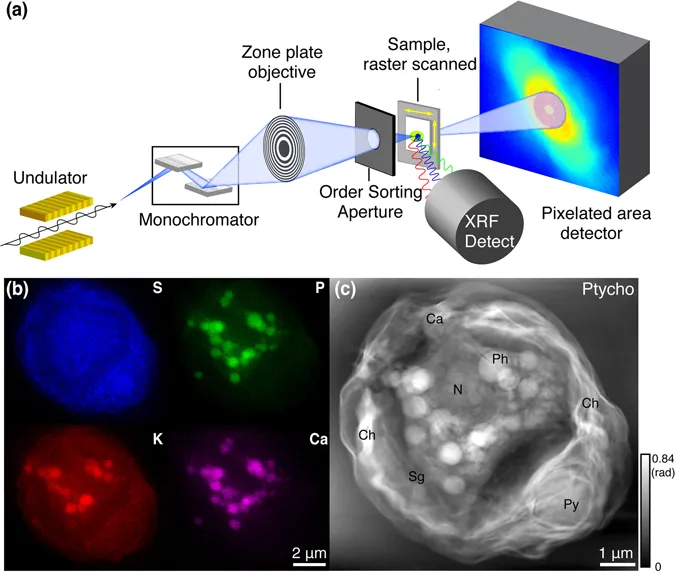
\includegraphics[scale=0.28]{junjing}
				\caption{Simultaenous Ptychography and fluoresence imaging \footnote{\cite{junjing}}}
			\end{figure}
		\end{center}	
	%\end{itemize}
\end{frame}


\begin{frame}{Factors affecting efficiency \& resolution}
	\begin{block}{}
		\begin{columns}[onlytextwidth,T]
			\column{\dimexpr\linewidth-30mm-10mm}
			\begin{itemize}
				\item Efficiency of zone plate depends on refractive index.
				\item Zones must be thick enough along beam direction to produce a phase shift of $\pi$, several um at hard x-ray energy.
				\item Spatial resolution limited to finest, outermost zone width.
			\end{itemize}
			\column{30mm}
			\begin{figure}
				\hspace*{-1.1cm}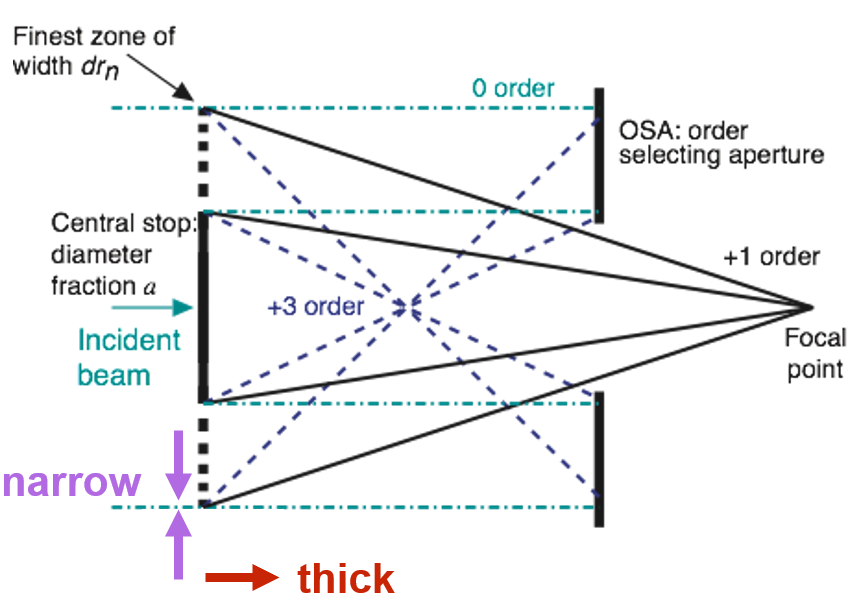
\includegraphics[width=50mm]{zp_chris}
				\caption{Thickness vs efficiency \footnotemark}
			\end{figure}
		\end{columns}
	\footnotetext{\cite{jacobsen_2019}}
	\end{block}
\end{frame}

\begin{frame}{Scalar theory is not enough}
	\begin{block}{}
		\begin{columns}[onlytextwidth,T]
			\column{\dimexpr\linewidth-30mm-10mm}
			\begin{itemize}
				\item Scalar approximation assumption $\rightarrow$ interaction between x-rays and the optic can be treated as one-step diffraction. 
				%\item This model fails to accurately describe the behavior of thick optics which start to have waveguide effects. 
				\item Clearly, waveguide effects need to be taken into account.
				\item Thick zone plate $\rightarrow$ test object.
				\item Klein-Cook param. : $Q_{K-C}$ indicator of 
				"diffraction regime"\footnotemark.
			\end{itemize}
			\column{30mm}
			\begin{figure}
				%\hspace*{-1cm}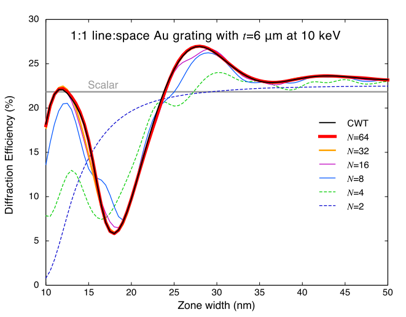
\includegraphics[width=50mm]{kenan}
				%\caption{Volume effects in 1d gratings \footnotemark}
				\hspace*{-1cm}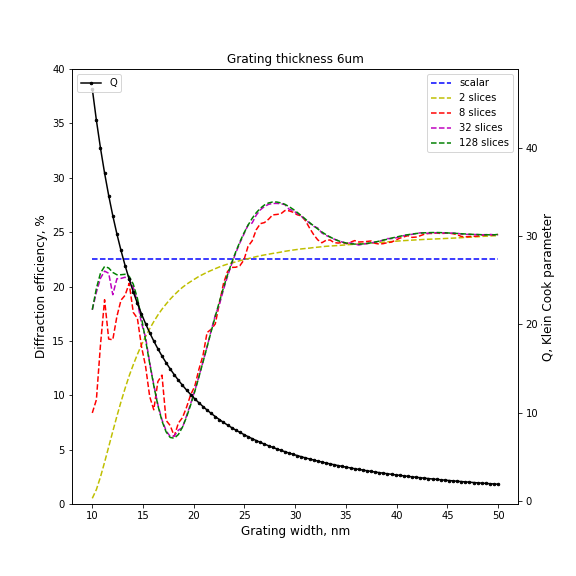
\includegraphics[width=50mm]{grating}
				\caption{Volume effects in 1d gratings}
			\end{figure}
		\end{columns}
	\footnotetext{\cite{QKC}}
	%\footnotetext{\cite{Li17}}
	\end{block}
\end{frame}


\section{Beyond Depth of Focus imaging}


\begin{frame}{What is DoF?}
\begin{itemize}
	\item Can be thought of as the longitudinal spread of focal spot
	\item Goes like $\approx5(\mbox{transverse res.})/\lambda^{2}$, 30nm/25keV$\rightarrow$90um.
\end{itemize}
	\begin{center}
		\begin{figure}
		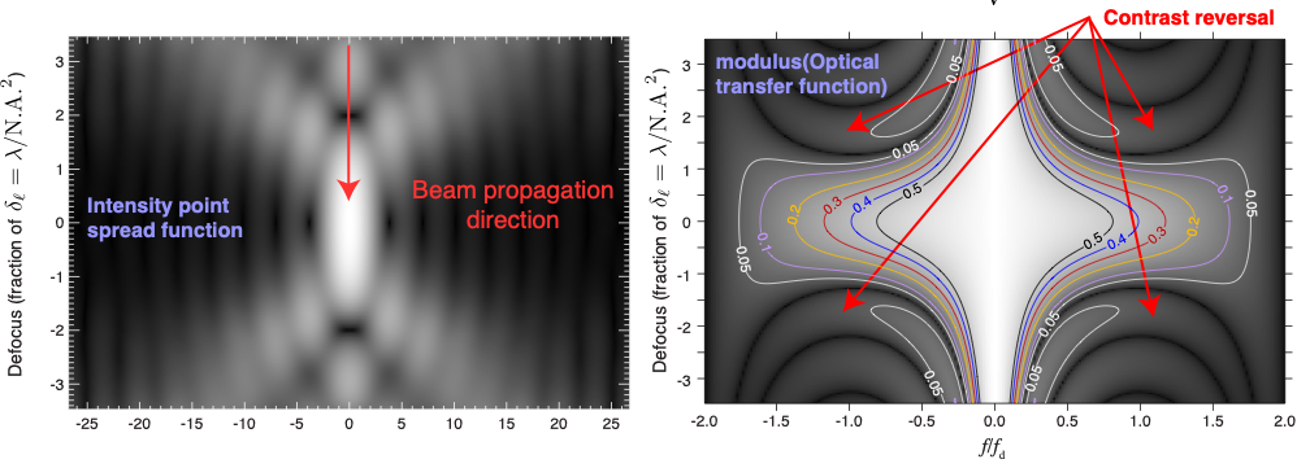
\includegraphics[scale=0.3]{dof}
		\caption{Optical Transfer Function in real and frequecny space \footnote{\cite{jacobsen_2019}}}	
		\end{figure}
	\end{center}
\end{frame}

\begin{frame}{Current Imaging schemes}
	\begin{itemize}
		\item Object within DoF
		\item No modulation of input wave within the object
	\end{itemize}
	\begin{center}
	\begin{figure}
		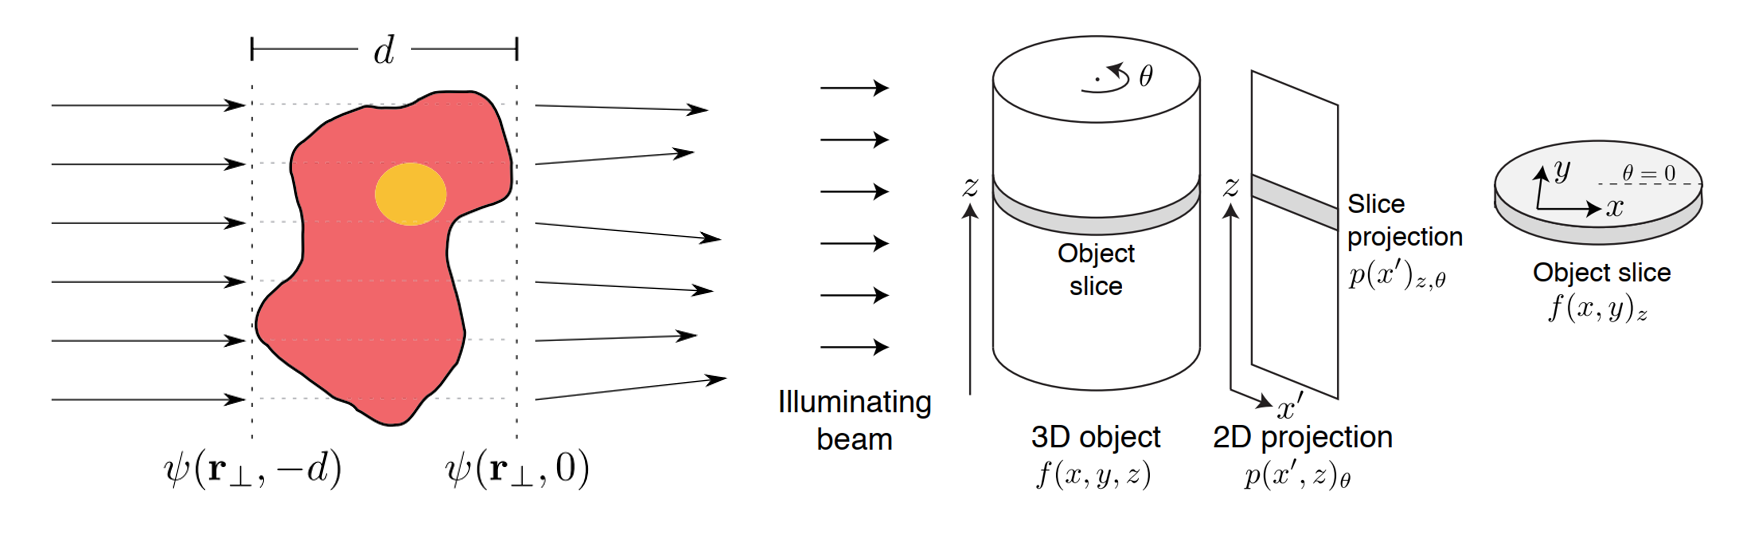
\includegraphics[scale=0.4]{ppa4}
			\caption{(Left) Pure Projection Approximation\footnote{\cite{Krenkel}}, (Right) Each slice is projected onto a 2D plane. All planes are independent of each other	\footnote{\cite{jacobsen_2019}}}
	\end{figure}
\end{center}


\end{frame}

\begin{frame}{Current Imaging schemes}
	%\begin{itemize}
	\begin{center}
		\begin{figure}
			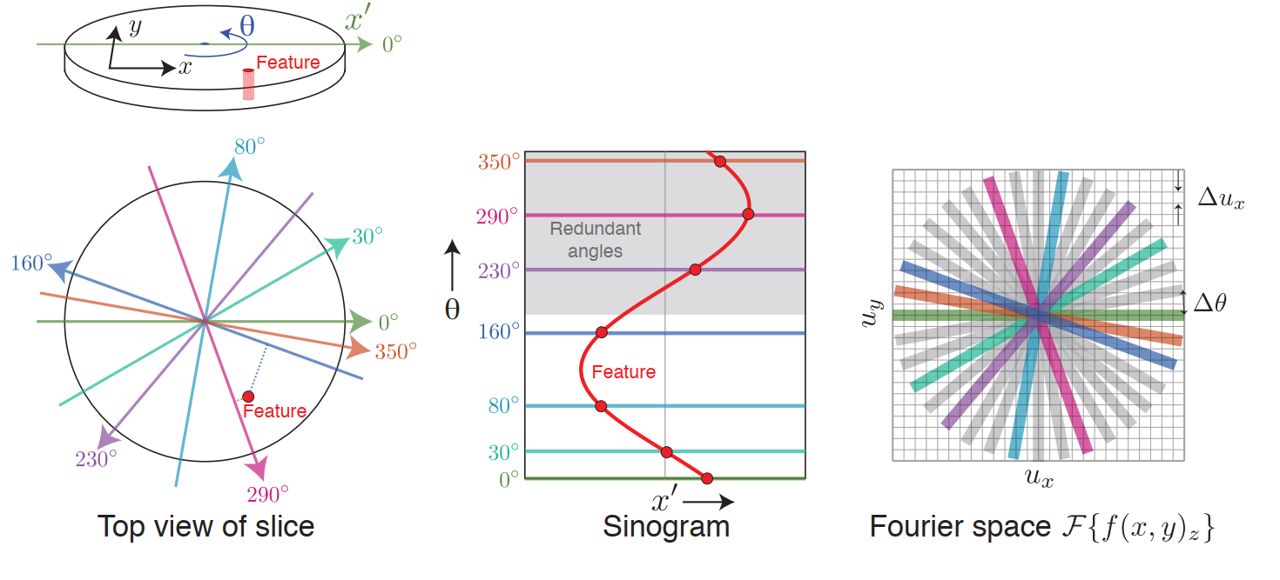
\includegraphics[scale=0.265]{ppa2}
			\caption{Spinning the object to obatin "sinograms", reconstruct each slice independently	\footnote{\cite{jacobsen_2019}}}
		\end{figure}
	\end{center}
	%\end{itemize}
\end{frame}

\begin{frame}{New reconstruction schemes}
\begin{itemize}
	\item "Thick" objects that extend beyond depth of focus $\rightarrow$ Pure Projection Approximation is not valid!
	\item New approaches $\rightarrow$ optimization of cost function\footnotemark,  neural networks\footnotemark, etc.
	\item We will compare the relative merits of two approaches to solve the forward problem.
\end{itemize}
\footnotetext{\cite{Gilles_18,Tsai_16,Ozturk_18,Shimomura_15,Li_2018}}
\footnotetext{\cite{Rivenson2018,Goy_Alexandre,FineupCNN,KamilovCNN}}
\end{frame}


\section{Multi-slice method}
\begin{frame}{Multislice}
	\begin{itemize}
		\item "Slice" the object into multiple thin sections.
		\footnote{\cite{ms_1957,VanRoey81,Li17}}.
		\item Agrees with rigorous coupled wave theory \footnote{\cite{Li17}}.
		\item At pixel $\approx0.25$ feature size, need $\approx Q_{K-C}$ steps.
	\end{itemize}
	\begin{center}
		\begin{figure}
			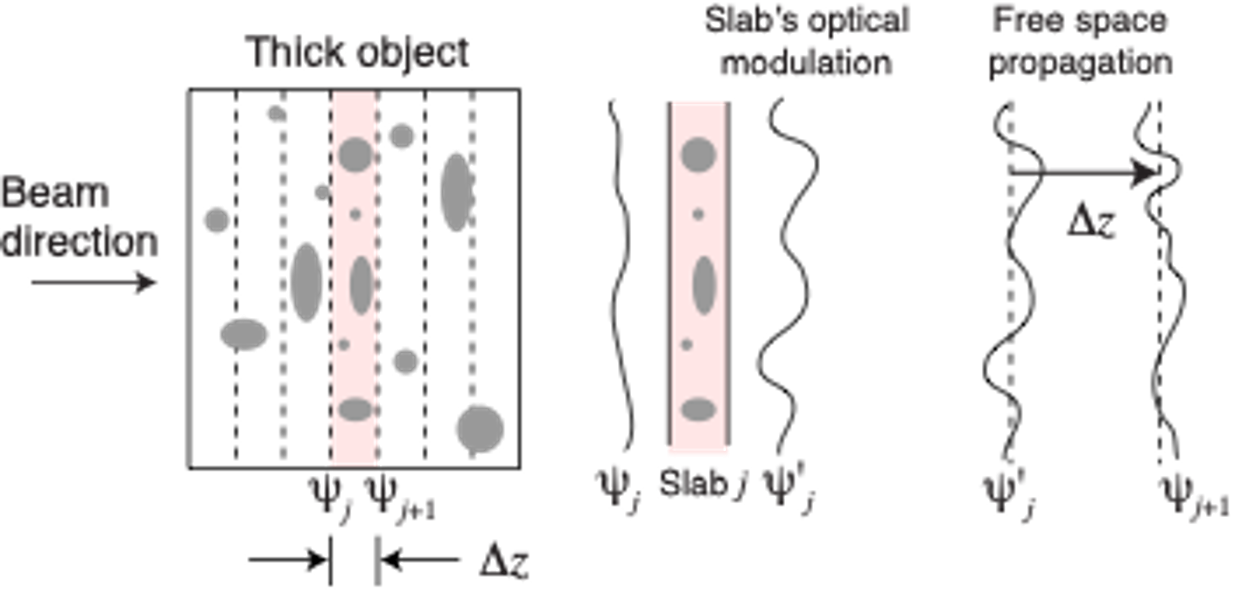
\includegraphics[scale=0.2275]{ms}
			\caption{Multi-slice schematic \footnote{\cite{jacobsen_2019}} }
		\end{figure}
	\end{center}
\end{frame}

\begin{frame}{Implementation}
	\begin{itemize}
		\item Slab modulation $\rightarrow$ point-wise multiply with the transmission matrix (a point-wise function of refractive indices)\footnote{\cite{ms_1957,VanRoey81,Li17}}.
		\item Free Space propagation is given by Fresnel Transform which is implemented numerically by \footnote{\cite{goodman_2017}}:
		\\~\\
		\qquad $\psi_{out}=\mathcal{F}^{-1}\{\mathcal{F}\psi_{in}*TF\}$
		\\~\\
		$TF(x,y) = exp(\dfrac{-i2\pi\delta z}{\lambda})\sqrt{1-\lambda^2(u_x^2+u_y^2)}$
		\\~\\
		\item Where $\lambda$ is wavelength, $\delta z$ is step size, $u_x/u_y$ are the x/y co-ordinates.	
	\end{itemize}
\end{frame}


\section{Finite Difference methods for wave propagation}

\begin{frame}{FD-basics}
	\begin{itemize}
		\item Directly solve the Helmholtz equation for scalar diffraction in inhomogenous matter: 
		 %$\nabla^{2}\psi+k^{2}n^{2}(x,y,z)\psi=0$
		\\~\\
		\qquad $\nabla^{2}\psi+k^{2}n^{2}(x,y,z)\psi=0$
		\\~\\
		($k=\frac{2\pi}{\lambda}$ and $n(x,y,z)$ is the refractive index)
		\item Approximate the wavefunction with plane wave and osciallating parts: 
		\\~\\ 
		\qquad $\psi(x,y,z) = u(x,y,z)exp(-ikz)$
		\\~\\
	\end{itemize}
\end{frame}

\begin{frame}{FD-basics}
	\begin{itemize}
		\item Substituting this in the Helmholtz equation and neglecting the derivative of u along the direction of propagation, we get the following equation :
		\\~\\
		\qquad	$\mbox{-2ik}\frac{\partial}{\partial z}u+(\frac{\partial ^{2}}{\partial x}+\frac{\partial ^{2}}{\partial y})u + k^{2}(n^{2}-1)=0$ 
		\\~\\
		\item Defining $a = \frac{-i}{2k}$ and $F(x,y,z) = \frac{-ik}{2}(n^{2}(x,y,z)-1)$; PDE now becomes \footnote{\cite{Fuhse_thesis,Kopylov}} :
		\\~\\
		\qquad $\frac{\partial u}{\partial z} = \mbox{a}(\frac{\partial ^{2}u}{\partial x^{2}}+\frac{\partial^{2}u}{\partial y^{2}}) + \mbox{F(x,y,z)}u$
		\\~\\
		\item In scaled units, u is $\approx1e^{1}$, $|a|$ is $\approx 1e^{2}$ and $|F|$ is $\approx 1e^{-3}$.
		%\item $|a|$ is $\approx 1e^{11}$ and $|F|$ is $\approx 1e^{6}$ , u is $\approx1e^{-9}$ (all in SI units).
	\end{itemize}
\end{frame}


\begin{frame}{Results from literature}
\begin{itemize}
	%\item Initial proof-of-concept implementations were in IDL \footnote{\cite{Kopylov,Fuhse_thesis}}.
	\item Need second-order integration along direction of propagation for accuracy \footnote{\cite{Fuhse_thesis,Melchior17}}.
	\item A recent implementation \footnote{\cite{Melchior17}} was in C\texttt{++} with a Python front end where ADI \footnote{\cite{BIRKHOFF1962189}} was used.
	\item Preferred method\footnote{\cite{Melchior17}} : 		
	\\
	free-space $\rightarrow$ MS,
	\\
	waveguides (inhomogenous matter) $\rightarrow$ FD 
\end{itemize}
\end{frame}

\section{PETSc Implementation}
	
\begin{frame}{PETSc Implementation \footnote{\url{https://github.com/s-sajid-ali/xwp_petsc}}}
\begin{itemize}
	\item For the FD method : Standard 5-point stencil.
	\\~\\
	\qquad	${DMDA + CN/GMRES/GAMG}$
	\\~\\
	\item For the MS method : Using the PETSc-FFTW interface which maps FFT/IFFT $\rightarrow$ MatMult,MatMultTranspose
	\\~\\
	\qquad	Loop $\{VecView/2DFFT/VecPointwiseMult/2DIFFT\}$
	\\~\\
	\item PETSc vastly simplifies parallel IO, pointwise mult and FFT integration!	
\end{itemize}
\end{frame}

\begin{frame}{Sensitivity sweep}
	\begin{itemize}
		\item Test a zone plate of size $2^{14} x 2^{14}$, $Q_{K-C}$ = 500. 
		\item Vary number of TS steps and KSP Rtol.
		\item A relative tolerance of $1e-5$ suffices!
		\begin{center}
		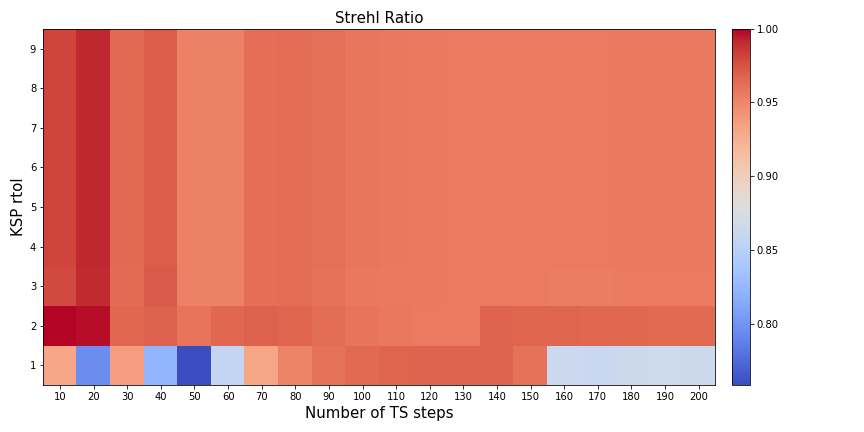
\includegraphics[scale=0.35]{sensitivity}
		\end{center}
		
	\end{itemize}
\end{frame}

\begin{frame}{Zone plate results}
	\begin{itemize}
		\item Test a zone plate of size $2^{15} x 2^{15}$; $Q_{K-C}$ = 1500.
	    \item FD converges in fewer steps, but needs more memory.
		\begin{center}
			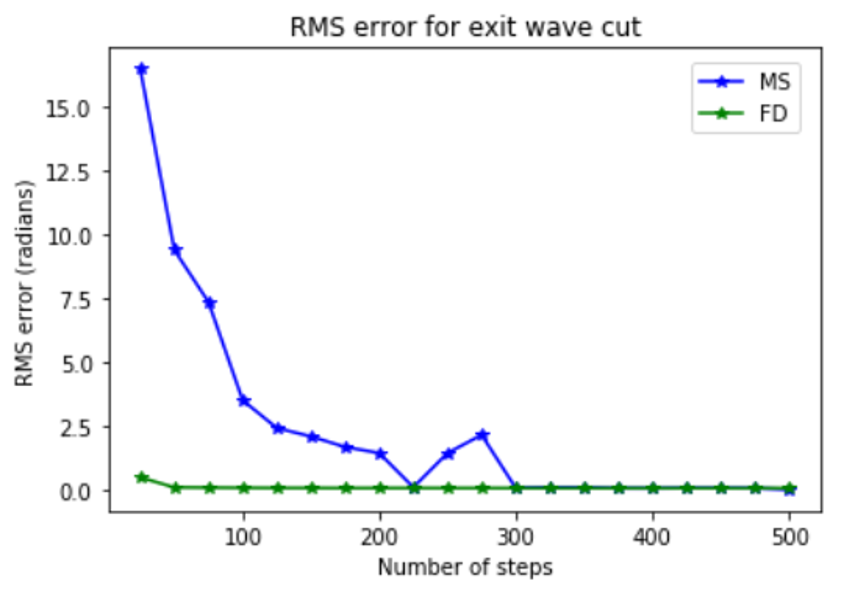
\includegraphics[scale=0.5]{fdms2}
		\end{center}
	\end{itemize}
\end{frame}

\begin{frame}{Zone plate results}
\begin{itemize}
	\item Test a zone plate of size $2^{15} x 2^{15}$, $Q_{K-C}$ = 1500.
	\begin{center}
		%\hspace*{-1.1cm}
		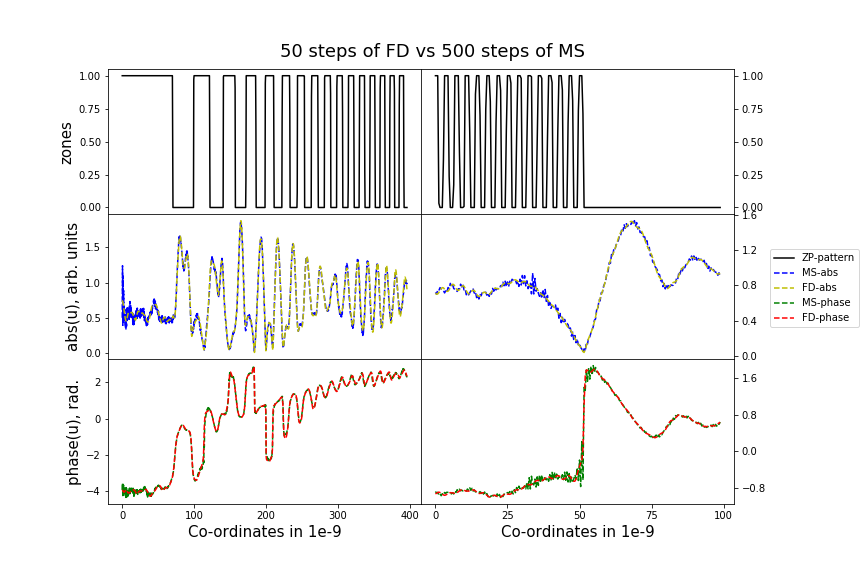
\includegraphics[scale=0.325]{fdms}
	\end{center}
\end{itemize}
\end{frame}


%\begin{frame}{Scaling}
%\begin{itemize}
%	\item ?
%\end{itemize}
%\end{frame}

\begin{frame}{Next Steps}
	\begin{itemize}
		%\item Implement a local convolution method for wave propagation. Again, DMDA vastly simplifies data management!
		\item Simulate tomography (essentially $MatMult$ + wave propagation); for $\theta_i\subset(0,\pi)$, $TS(A_{\theta_i}*x)\rightarrow y_{\theta_i}$.
		\item Solve the inverse problem with $TAO$ using adjoints given by $TSAdjoint$; Given $y_{\theta_i}'s \mbox{ for }  \theta_i\subset(0,\pi)$ get $x$!
	\end{itemize}
\end{frame}

%\begin{comment}
% Placing a * after \section means it will not show in the
% outline or table of contents.

\begin{frame}{Acknowledgements}
  \begin{itemize}
  \item \alert{Barry Smith} MCS,ANL
  \item \alert{Hong Zhang} MCS,ANL.
  \item \alert{PETSc Developers} on petsc-users \& petsc-maint.
  \item \alert{bebop-LCRC} ANL \& \alert{theta-ALCF} ANL.
  \item \alert{NIMH} U01 MH109100 \& \alert{ANL-LDRD}.
  \end{itemize}
\end{frame}

%\end{comment}

% All of the following is optional and typically not needed. 
%\appendix
\renewcommand*{\bibfont}{\scriptsize}
\begin{frame}[t, allowframebreaks]
\frametitle{References}
\bibliographystyle{dinat-etal}
\bibliography{petsc_19}
\end{frame}

\end{document}

